\documentclass{article}
\usepackage{tikz}

\begin{document}

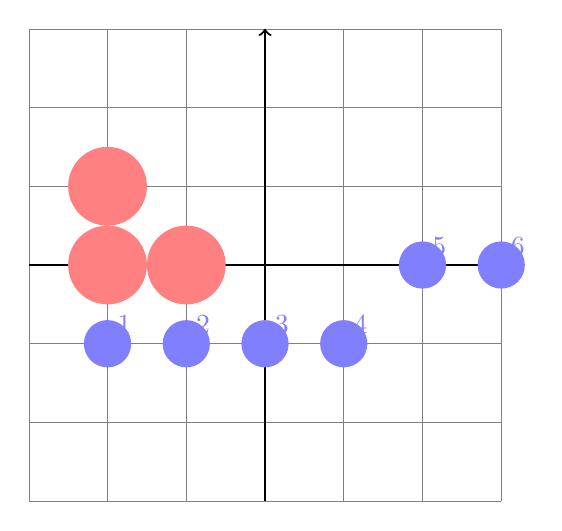
\begin{tikzpicture}[scale=1]
    % Draw the grid
    \draw[help lines] (0,0) grid (6,6);
    
    % Draw the arrows
    \draw[->, thick] (0,3) -- (6,3);
    \draw[->, thick] (3,0) -- (3,6);
    
    % Draw the circles with numbers
    \foreach \x/\y/\num in {1/2/1, 2/2/2, 3/2/3, 4/2/4, 5/3/5, 6/3/6} {
        \fill[blue!50] (\x,\y) circle (0.3) node[above right] {\num};
    }
    
    % Draw the red circles
    \fill[red!50] (2,3) circle (0.5);
    \fill[red!50] (1,3) circle (0.5);
    \fill[red!50] (1,4) circle (0.5);
\end{tikzpicture}

\end{document}